\clearpage
\subsection{Graph Transformations and Numerical Checks}
\label{sec:graph-cases}

\begin{table}[!htbp]
\centering\scriptsize
\caption{Reference graph transformations and observable outputs for five
extension tasks. Coral marks matched operations, teal the replacement, and
blue typed inputs. Graphs and values show the task contracts' expected results.
RNE denotes round-to-nearest, ties-to-even.}
\label{tab:graph-cases}
\setlength{\tabcolsep}{5pt}
\renewcommand{\arraystretch}{1.15}
\begin{tabular}{@{}>{\centering\arraybackslash}m{\dimexpr0.5\textwidth-5pt\relax}>{\centering\arraybackslash}m{\dimexpr0.5\textwidth-5pt\relax}@{}}
\toprule
Before & After \\
\midrule
\multicolumn{2}{@{}p{\textwidth}@{}}{\textbf{Remove add-by-zero.}\quad\texttt{rew-add-zero}\par
f32[4], positive zero, \texttt{no\_signed\_zeros}. All users now read
\texttt{\%x}; adding 0.001 retains the add.} \\*[2pt]
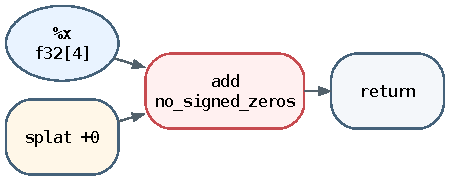
\includegraphics[width=6.4cm,height=1.65cm,keepaspectratio]{figures/task-zero-before.pdf} &
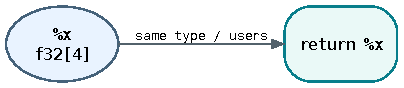
\includegraphics[width=6.4cm,height=1.65cm,keepaspectratio]{figures/task-zero-after.pdf} \\[5pt]
\midrule
\multicolumn{2}{@{}p{\textwidth}@{}}{\textbf{Cancel a lossless cast round trip.}\quad\texttt{rew-redundant-cast}\par
i8$\to$i16$\to$i8 preserves \texttt{[-128,-1,0,127]}.
i16$\to$i8$\to$i16 retains both casts.} \\*[2pt]
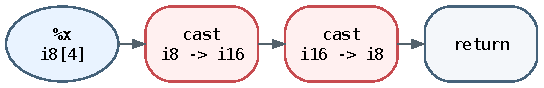
\includegraphics[width=6.4cm,height=1.65cm,keepaspectratio]{figures/task-cast-before.pdf} &
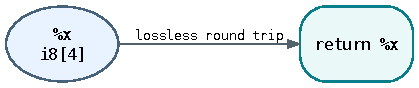
\includegraphics[width=6.4cm,height=1.65cm,keepaspectratio]{figures/task-cast-after.pdf} \\[5pt]
\midrule
\multicolumn{2}{@{}p{\textwidth}@{}}{\textbf{Expand GELU.}\quad\texttt{con-gelu-expand}\par
$y=0.5x(1+\operatorname{erf}(x/\sqrt{2}))$. Preserve f32[5] and every
output user; reject integer inputs.} \\*[2pt]
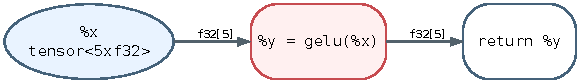
\includegraphics[width=6.4cm,height=1.65cm,keepaspectratio]{figures/agent-gelu-before.pdf} &
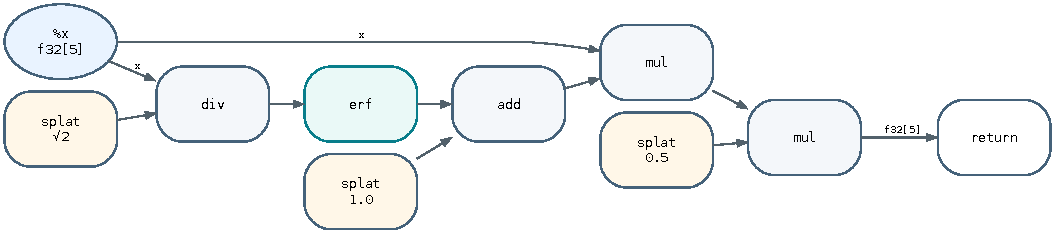
\includegraphics[width=6.4cm,height=1.65cm,keepaspectratio]{figures/agent-gelu-after.pdf} \\[5pt]
\midrule
\multicolumn{2}{@{}p{\textwidth}@{}}{\textbf{Expand quantized addition.}\quad\texttt{con-quant-expand}\par
\texttt{[-3,0,5,120]+[2,1,-8,120]} $\to$ \texttt{[-1,1,-3,127]};
all scales 0.5 and zero points 0. Reject negative scales.} \\*[2pt]
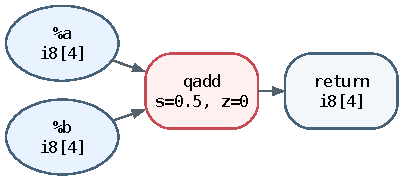
\includegraphics[width=6.4cm,height=1.65cm,keepaspectratio]{figures/task-quant-before.pdf} &
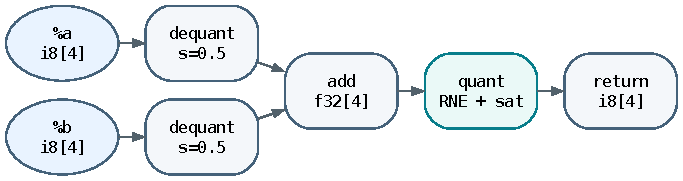
\includegraphics[width=6.4cm,height=1.65cm,keepaspectratio]{figures/task-quant-after.pdf} \\[5pt]
\midrule
\multicolumn{2}{@{}p{\textwidth}@{}}{\textbf{Fuse a single-use quantized chain.}\quad\texttt{vert-fused-op}\par
\texttt{x=[1,-2], w=[2,-3]}, bias 1; accumulator 9, scales 0.25/0.5:
RNE(4.5)$=4$. Shared convolution results retain the original chain.} \\*[2pt]
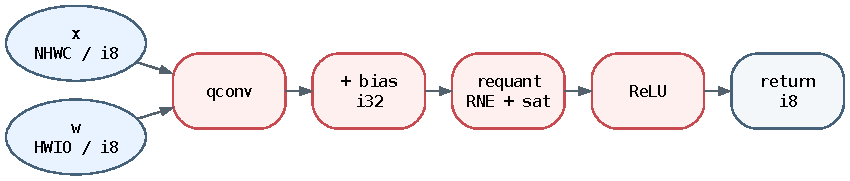
\includegraphics[width=6.4cm,height=1.65cm,keepaspectratio]{figures/task-fusion-before.pdf} &
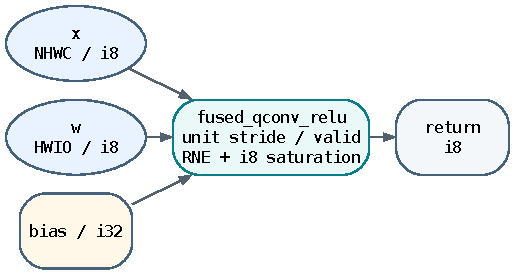
\includegraphics[width=6.4cm,height=1.65cm,keepaspectratio]{figures/task-fusion-after.pdf} \\[5pt]
\bottomrule
\end{tabular}
\end{table}

\begin{table}[!htbp]
\centering\scriptsize
\caption{Worked analysis and artifact-output checks. Values are task-contract
expectations; byte strings are hexadecimal.}
\label{tab:worked-outputs}
\setlength{\tabcolsep}{5pt}
\renewcommand{\arraystretch}{1.2}
\begin{tabular}{@{}p{2.6cm}p{4.2cm}p{4.7cm}p{5.0cm}@{}}
\toprule
Task / case & Input & Intermediate computation & Expected observable output \\
\midrule
Broadcast / empty axis &
\texttt{[2,0]}, \texttt{[1]} &
Align \texttt{[2,0]} with \texttt{[1,1]} &
legal; shape \texttt{[2,0]} \\
Interval / mixed product &
\texttt{[-2,3]} $\times$ \texttt{[-4,5]} &
Endpoint products \texttt{[8,-10,-12,15]} &
interval \texttt{[-12,15]} \\
Interval / add then ReLU &
\texttt{[-3,2] + [1,4]} &
Sum \texttt{[-2,6]}, then clamp below at 0 &
interval \texttt{[0,6]} \\
Manifest / repeated edges &
\texttt{add(arg,arg)};\par return \texttt{[twice,arg,twice]} &
\texttt{arg=v0}, \texttt{twice=v1}, node \texttt{n0} &
inputs \texttt{[v0,v0]};\par outputs \texttt{[v1,v0,v1]} \\
Wrapper / affine &
f32 \texttt{[-2,0,1.5,4]} &
Separate f32 multiply by 2, then add 1 &
\texttt{[-3,1,4,9]}; same result in-place \\
qint4 / odd count &
\texttt{[-8,-1,0,3,7]} $+$ \texttt{[1,1,-2,6,7]} &
i8 sums \texttt{[-7,0,-2,9,14]}; saturate &
\texttt{[-7,0,-2,7,7]}; bytes \texttt{09 7e 07} \\
qint4 / negative tail &
\texttt{[-8] + [-8]} &
Saturate $-16$ to $-8$; zero high nibble &
\texttt{[-8]}; byte \texttt{08} \\
\bottomrule
\end{tabular}
\end{table}
